
\documentclass[10pt]{report}
\usepackage{epsf}
\usepackage{amsmath}
\usepackage{amssymb}
\usepackage{palatino}
\usepackage[pdftex]{graphics}
\usepackage{fancyhdr}
\usepackage{epsfig}
\usepackage{multirow}
\usepackage{multicol}
\usepackage{cancel}
\usepackage{hyperref}
\usepackage{longtable}
\usepackage{ulem}
\usepackage[yyyymmdd]{datetime}
\renewcommand{\dateseparator}{-}
%\usepackage{draftwatermark}
\usepackage{listings}

\parindent 0in
\parskip 1ex
\oddsidemargin  0in
\evensidemargin 0in
\textheight 8.5in
\textwidth 6.5in
\topmargin -0.25in

\pagestyle{fancy}
\lhead{\textbf{\leftheader}}
\rhead{\textbf{\rightheader}}
\lfoot{Compiled: \today\ \currenttime}
\cfoot{}
\rfoot{\thepage}

\newcommand{\leftheader}{BME290L: MedTech Prototyping Skills}
\newcommand{\rightheader}{Palmeri (Spring 2023)}

\begin{document}

\section*{Lab 03: Advanced CAD - Hybrid III 6yo} 

    \begin{itemize}
        \item Create all of the parts for the Hybrid III 6yo test setup based on
        the attached drawings.  You should create all of these parts and their
        associated drawings and assemblies as part of the same ``Document'' and
        share that document with Dr. Palmeri and the TAs.
        \item Create the mechanical drawings associated with each of those parts
        (i.e., recreate the drawings that you are using to generate the parts)
        and the assembly.
        \item Assemble your parts as guided by the assembly diagram and as
            shown in the uploaded animation.  There are online tutorials on
            Assemblies if you need some refreshers:
            \begin{itemize}
                \item \url{https://learn.onshape.com/courses/introduction-to-assembly-design}
                \item \url{https://learn.onshape.com/courses/fundamentals-onshape-assemblies}
            \end{itemize}
        \item A explosion video of the assembled parts is shown here: \url{https://gitlab.oit.duke.edu/mlp6/MedTech-Prototyping-Skills/-/blob/main/labs/03-Hybrid-III-6yo/Assembly_v10.avi}
        \item Export and concatenate PDFs for all of your drawings, screenshots
        of your part generation steps, and upload them to Gradescope.
        \item Please feel free to ask questions via Teams!
    \end{itemize}

\centerline{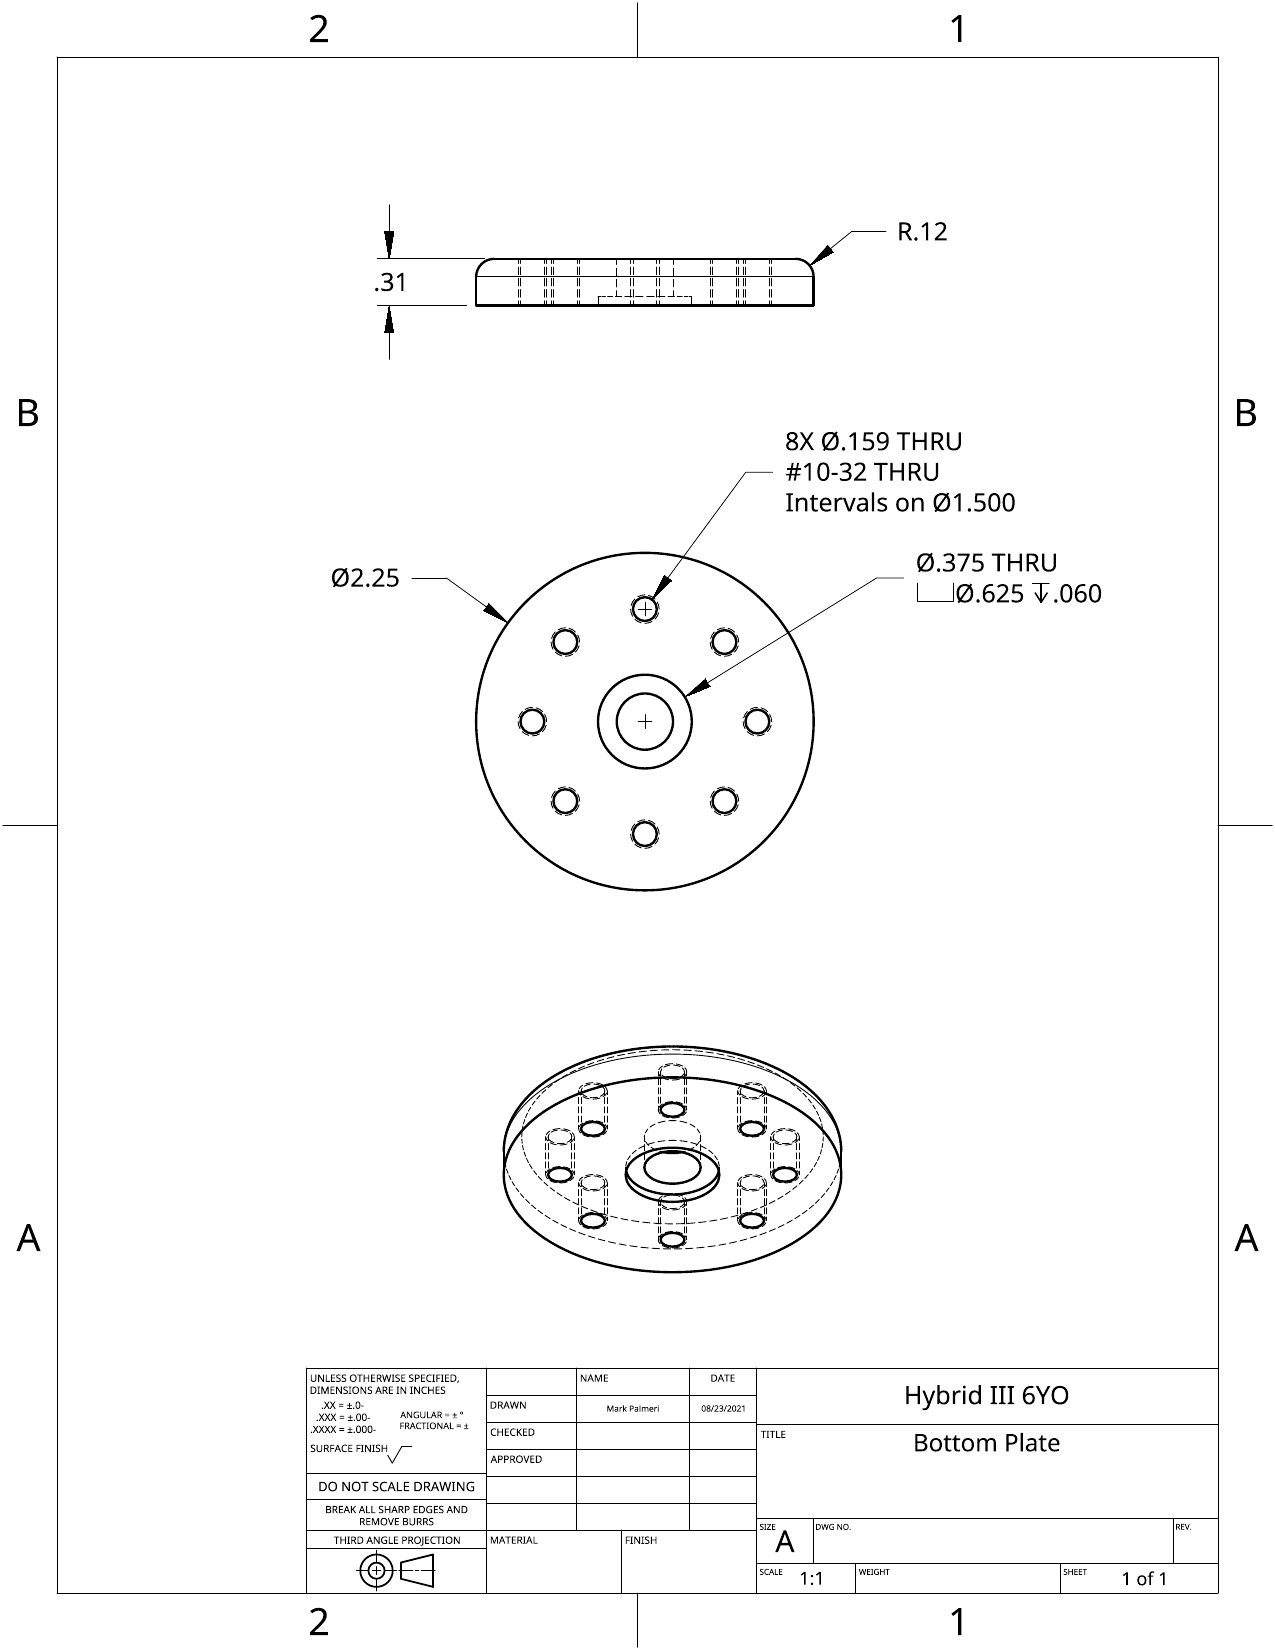
\includegraphics[width=1.0\textwidth]{BottomPlateDrawing.png}}
\centerline{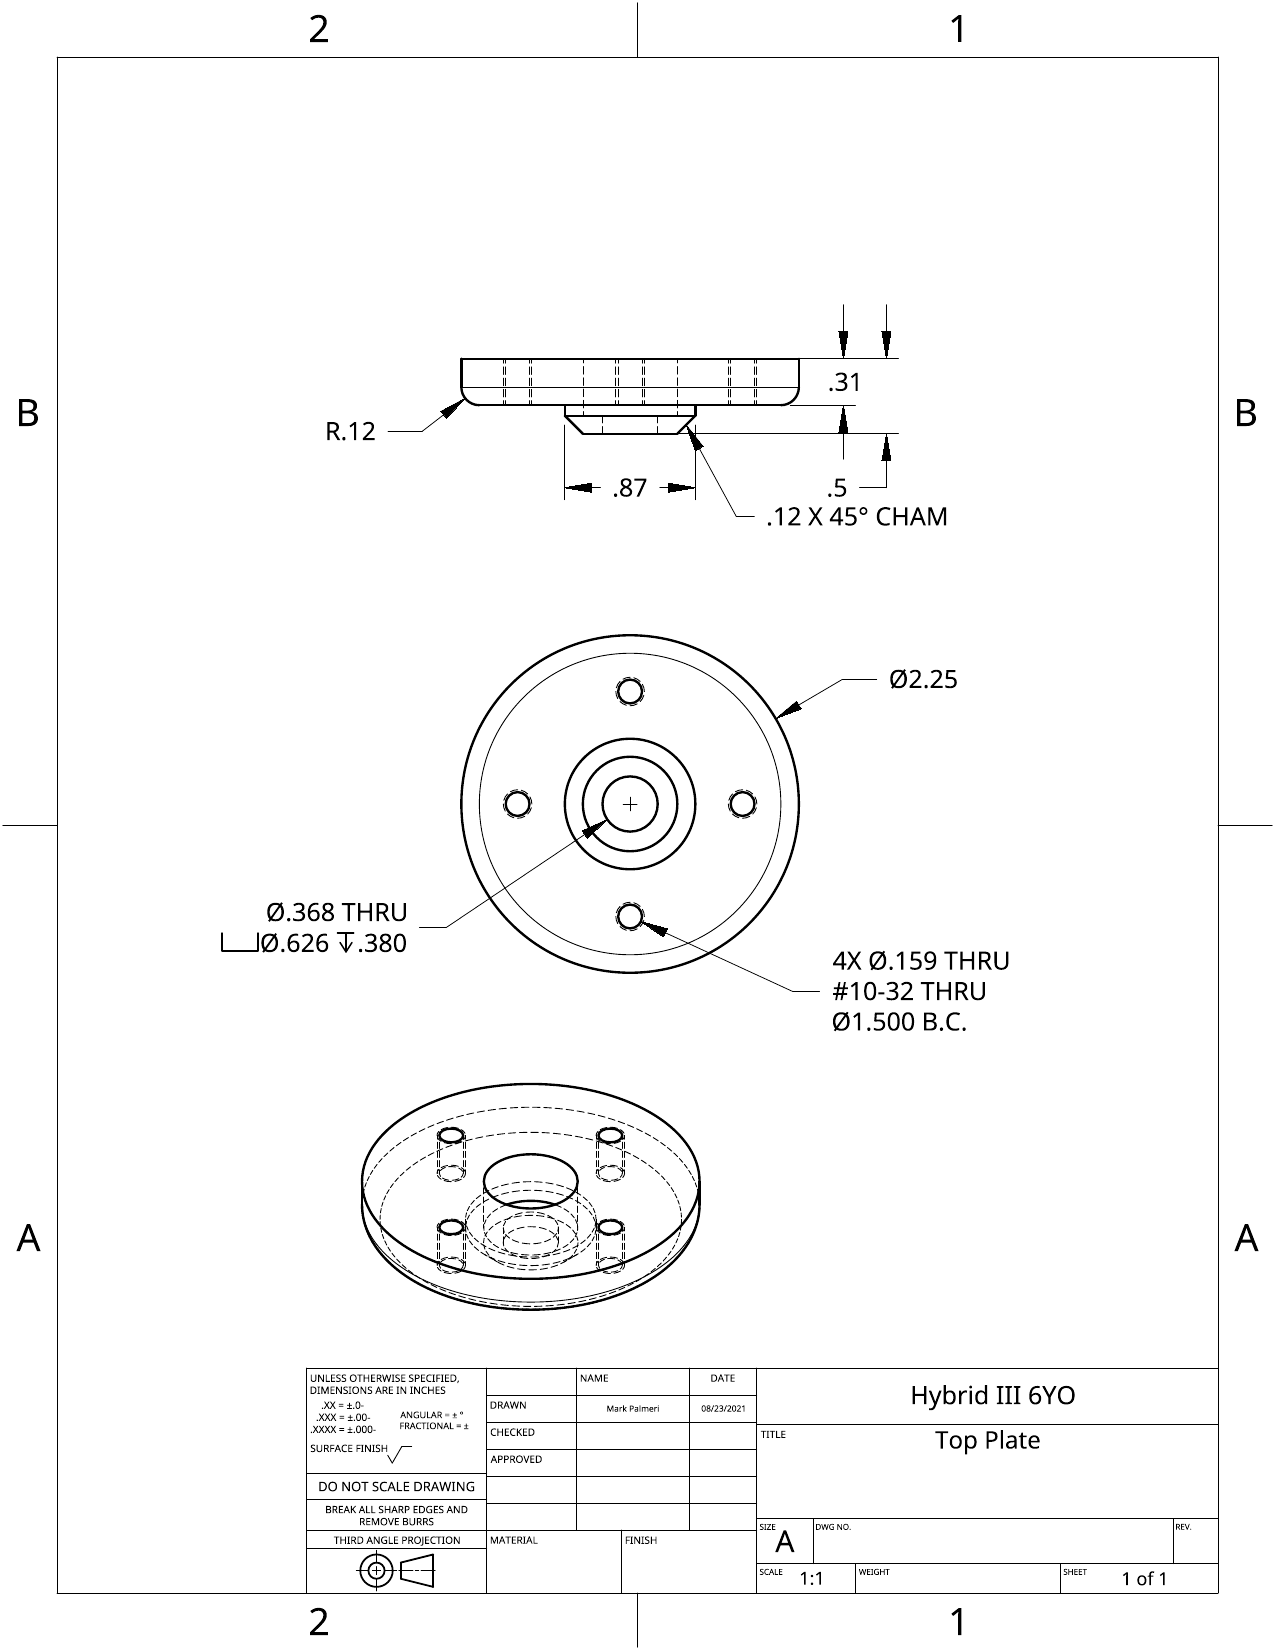
\includegraphics[width=1.0\textwidth]{TopPlateDrawing.png}}
\centerline{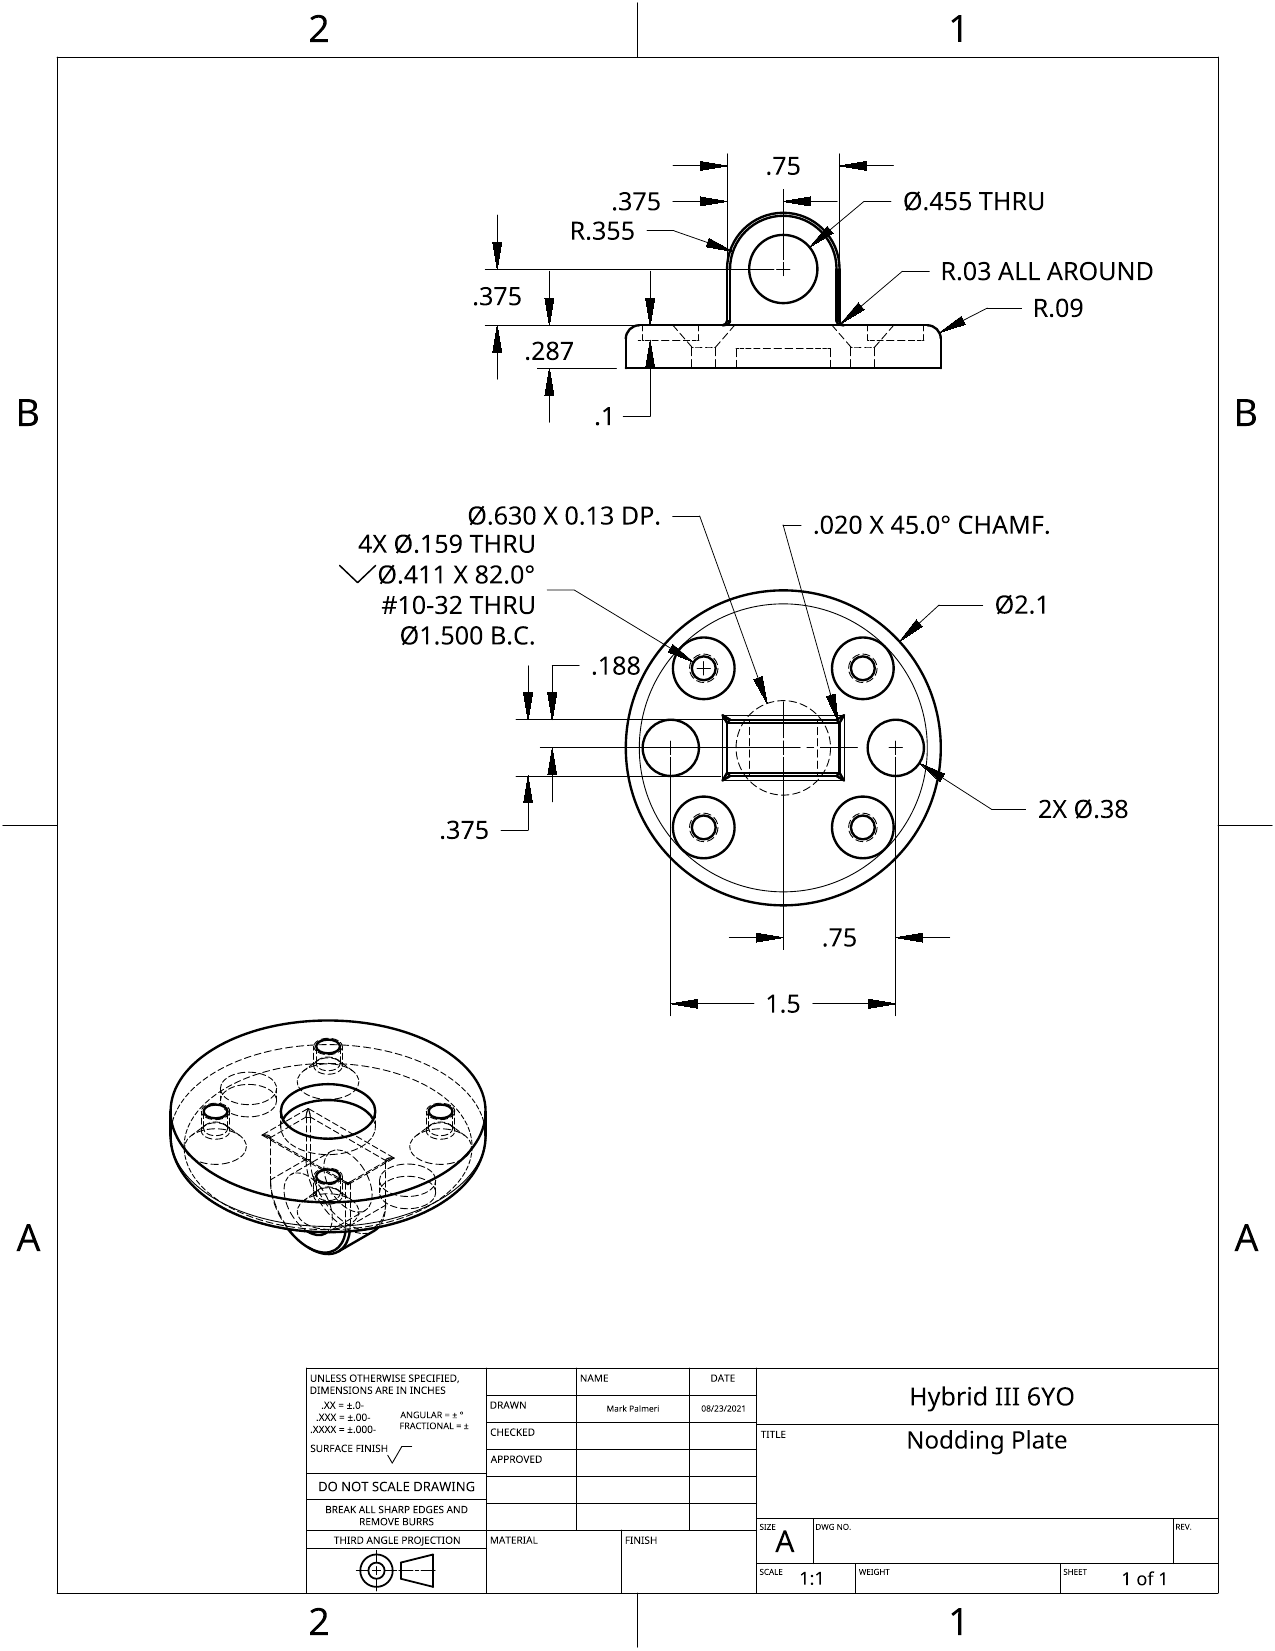
\includegraphics[width=1.0\textwidth]{NoddingPlateDrawing.png}}
\centerline{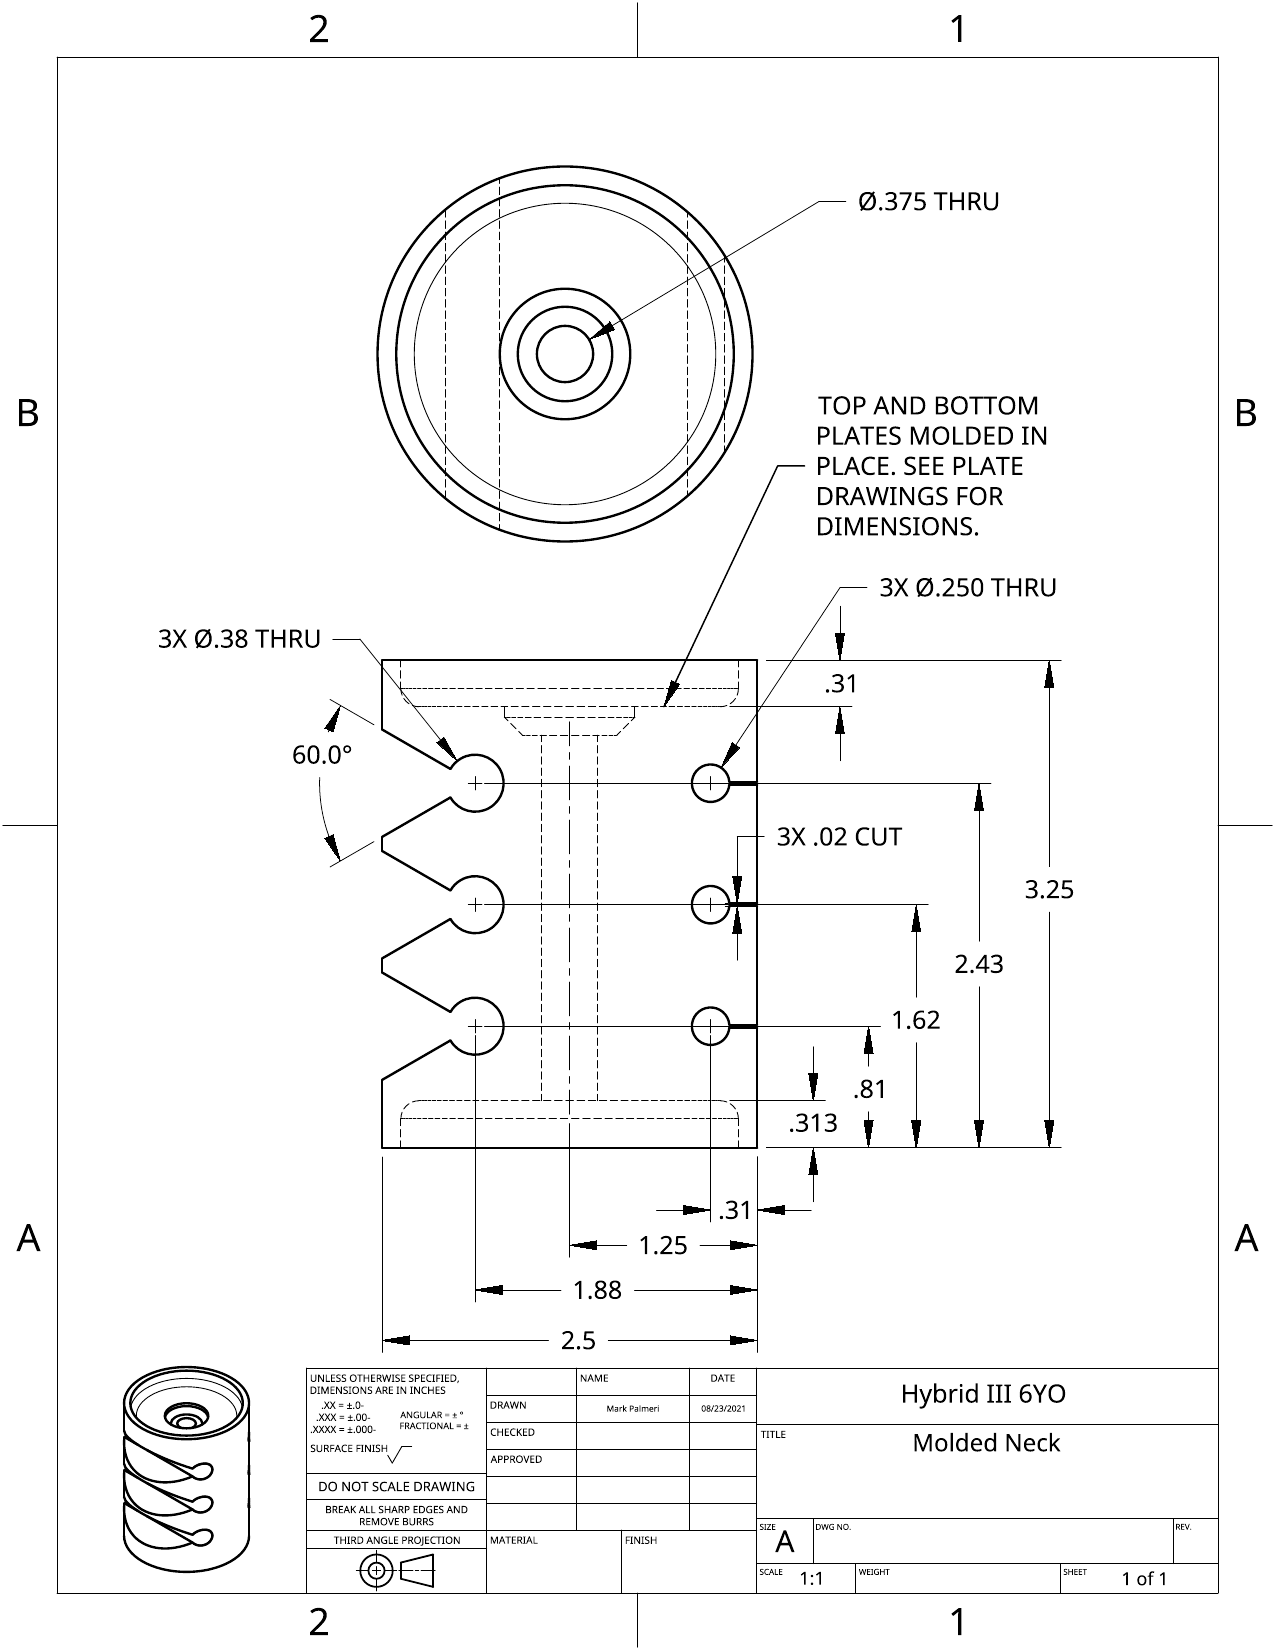
\includegraphics[width=1.0\textwidth]{MoldedNeckDrawing.png}}
\centerline{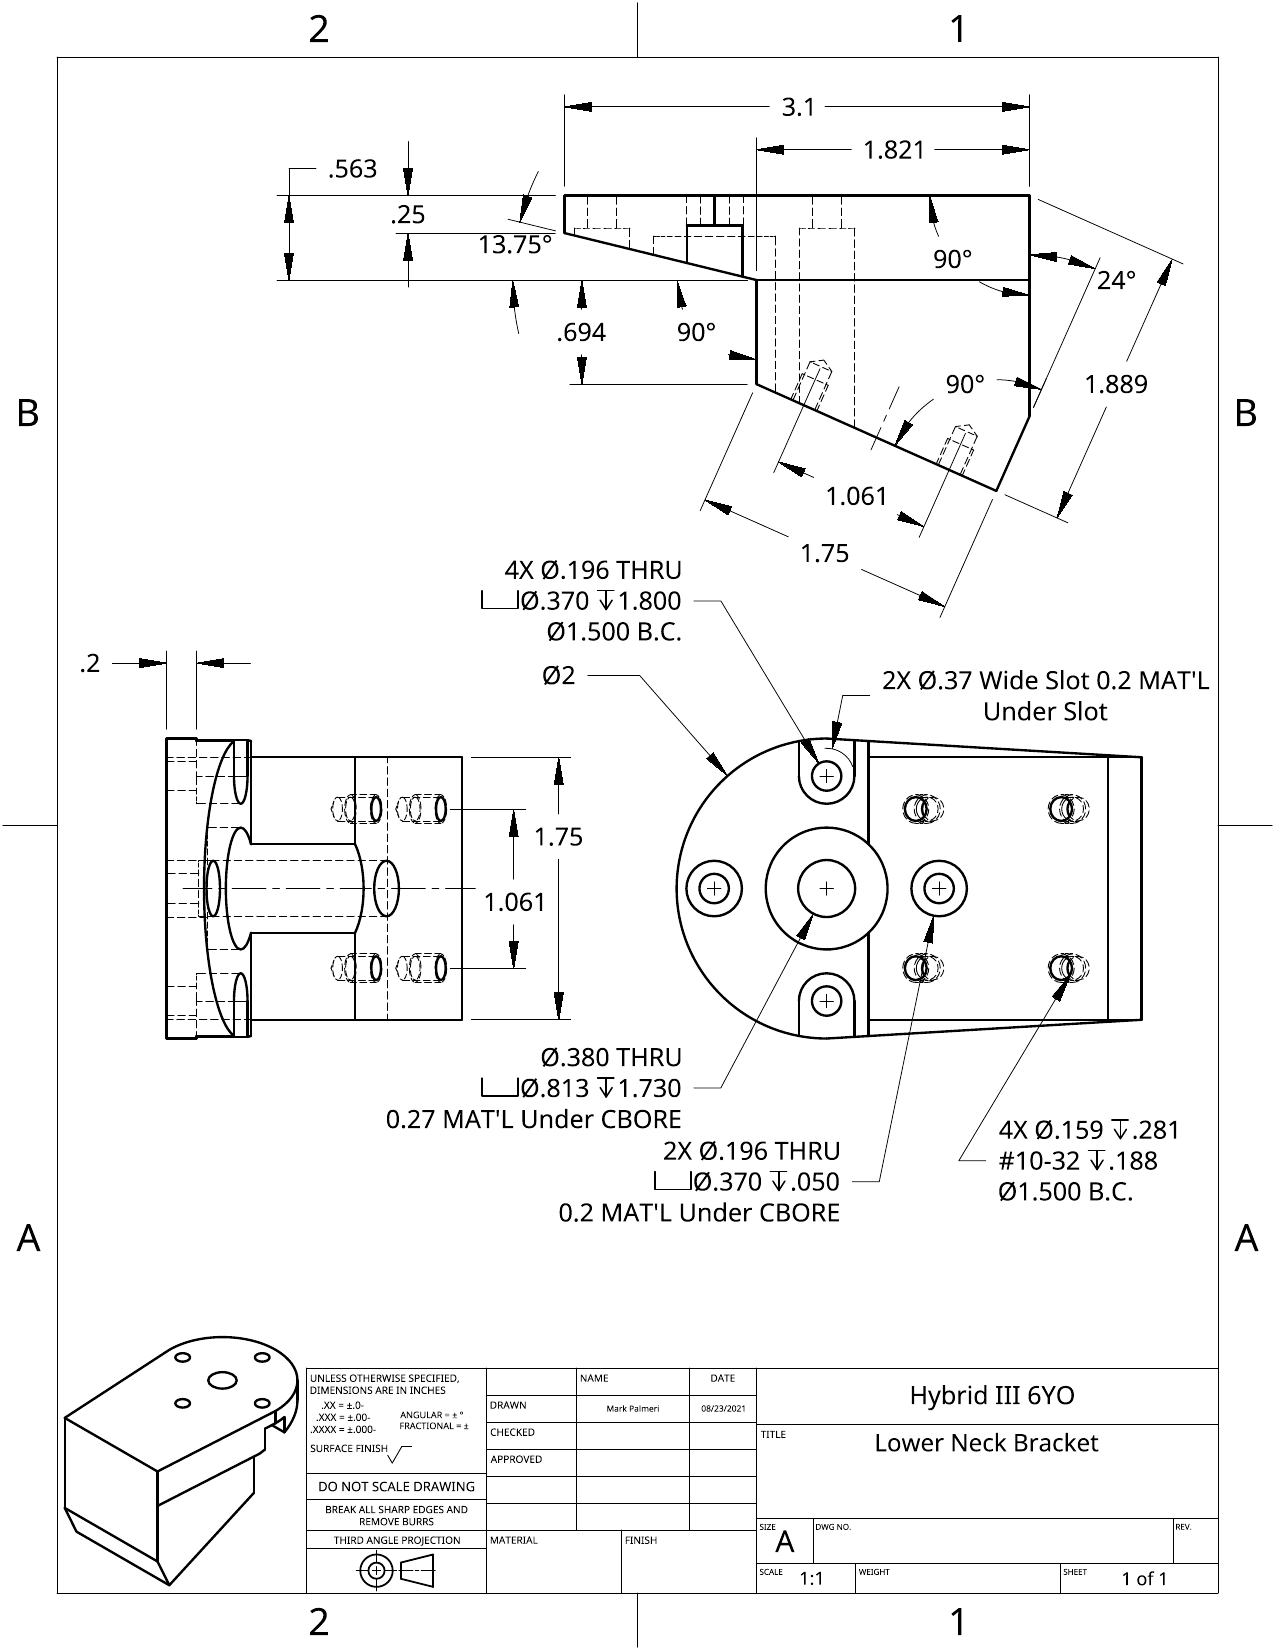
\includegraphics[width=1.0\textwidth]{LowerNeckBracketDrawing.png}}
\centerline{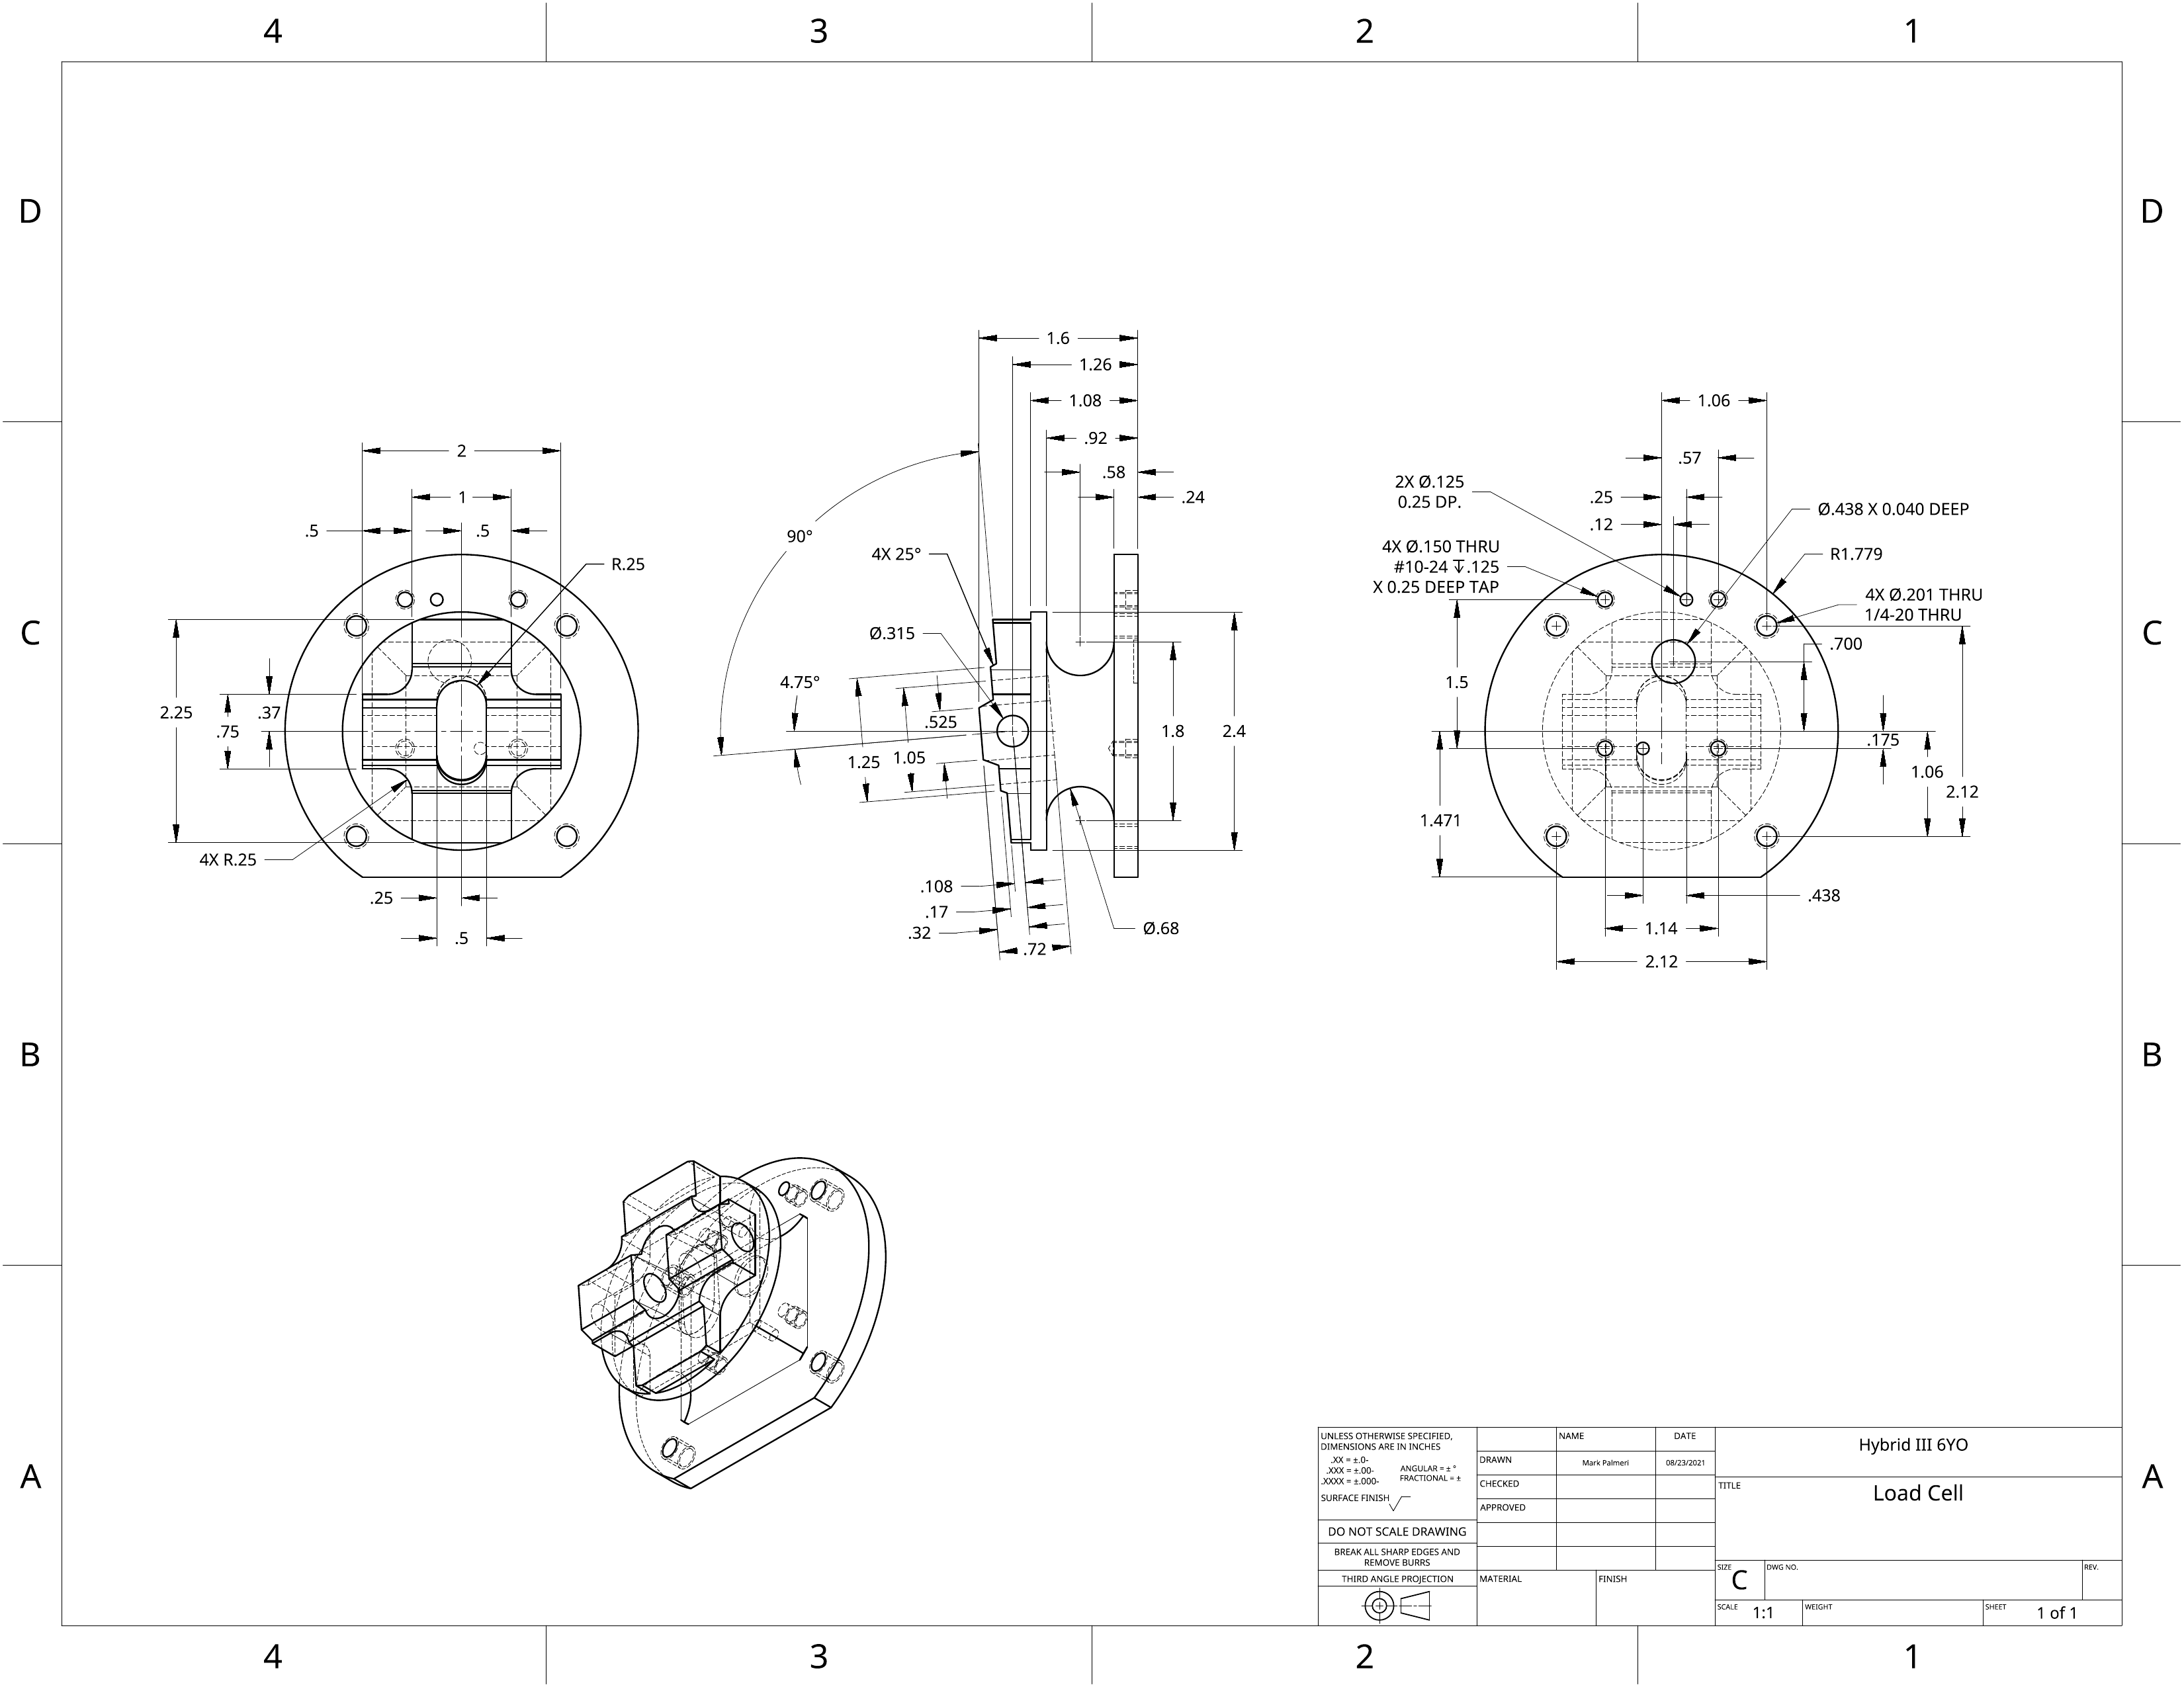
\includegraphics[angle=90,origin=c,width=1.0\textwidth]{LoadCellDrawing.png}}
\centerline{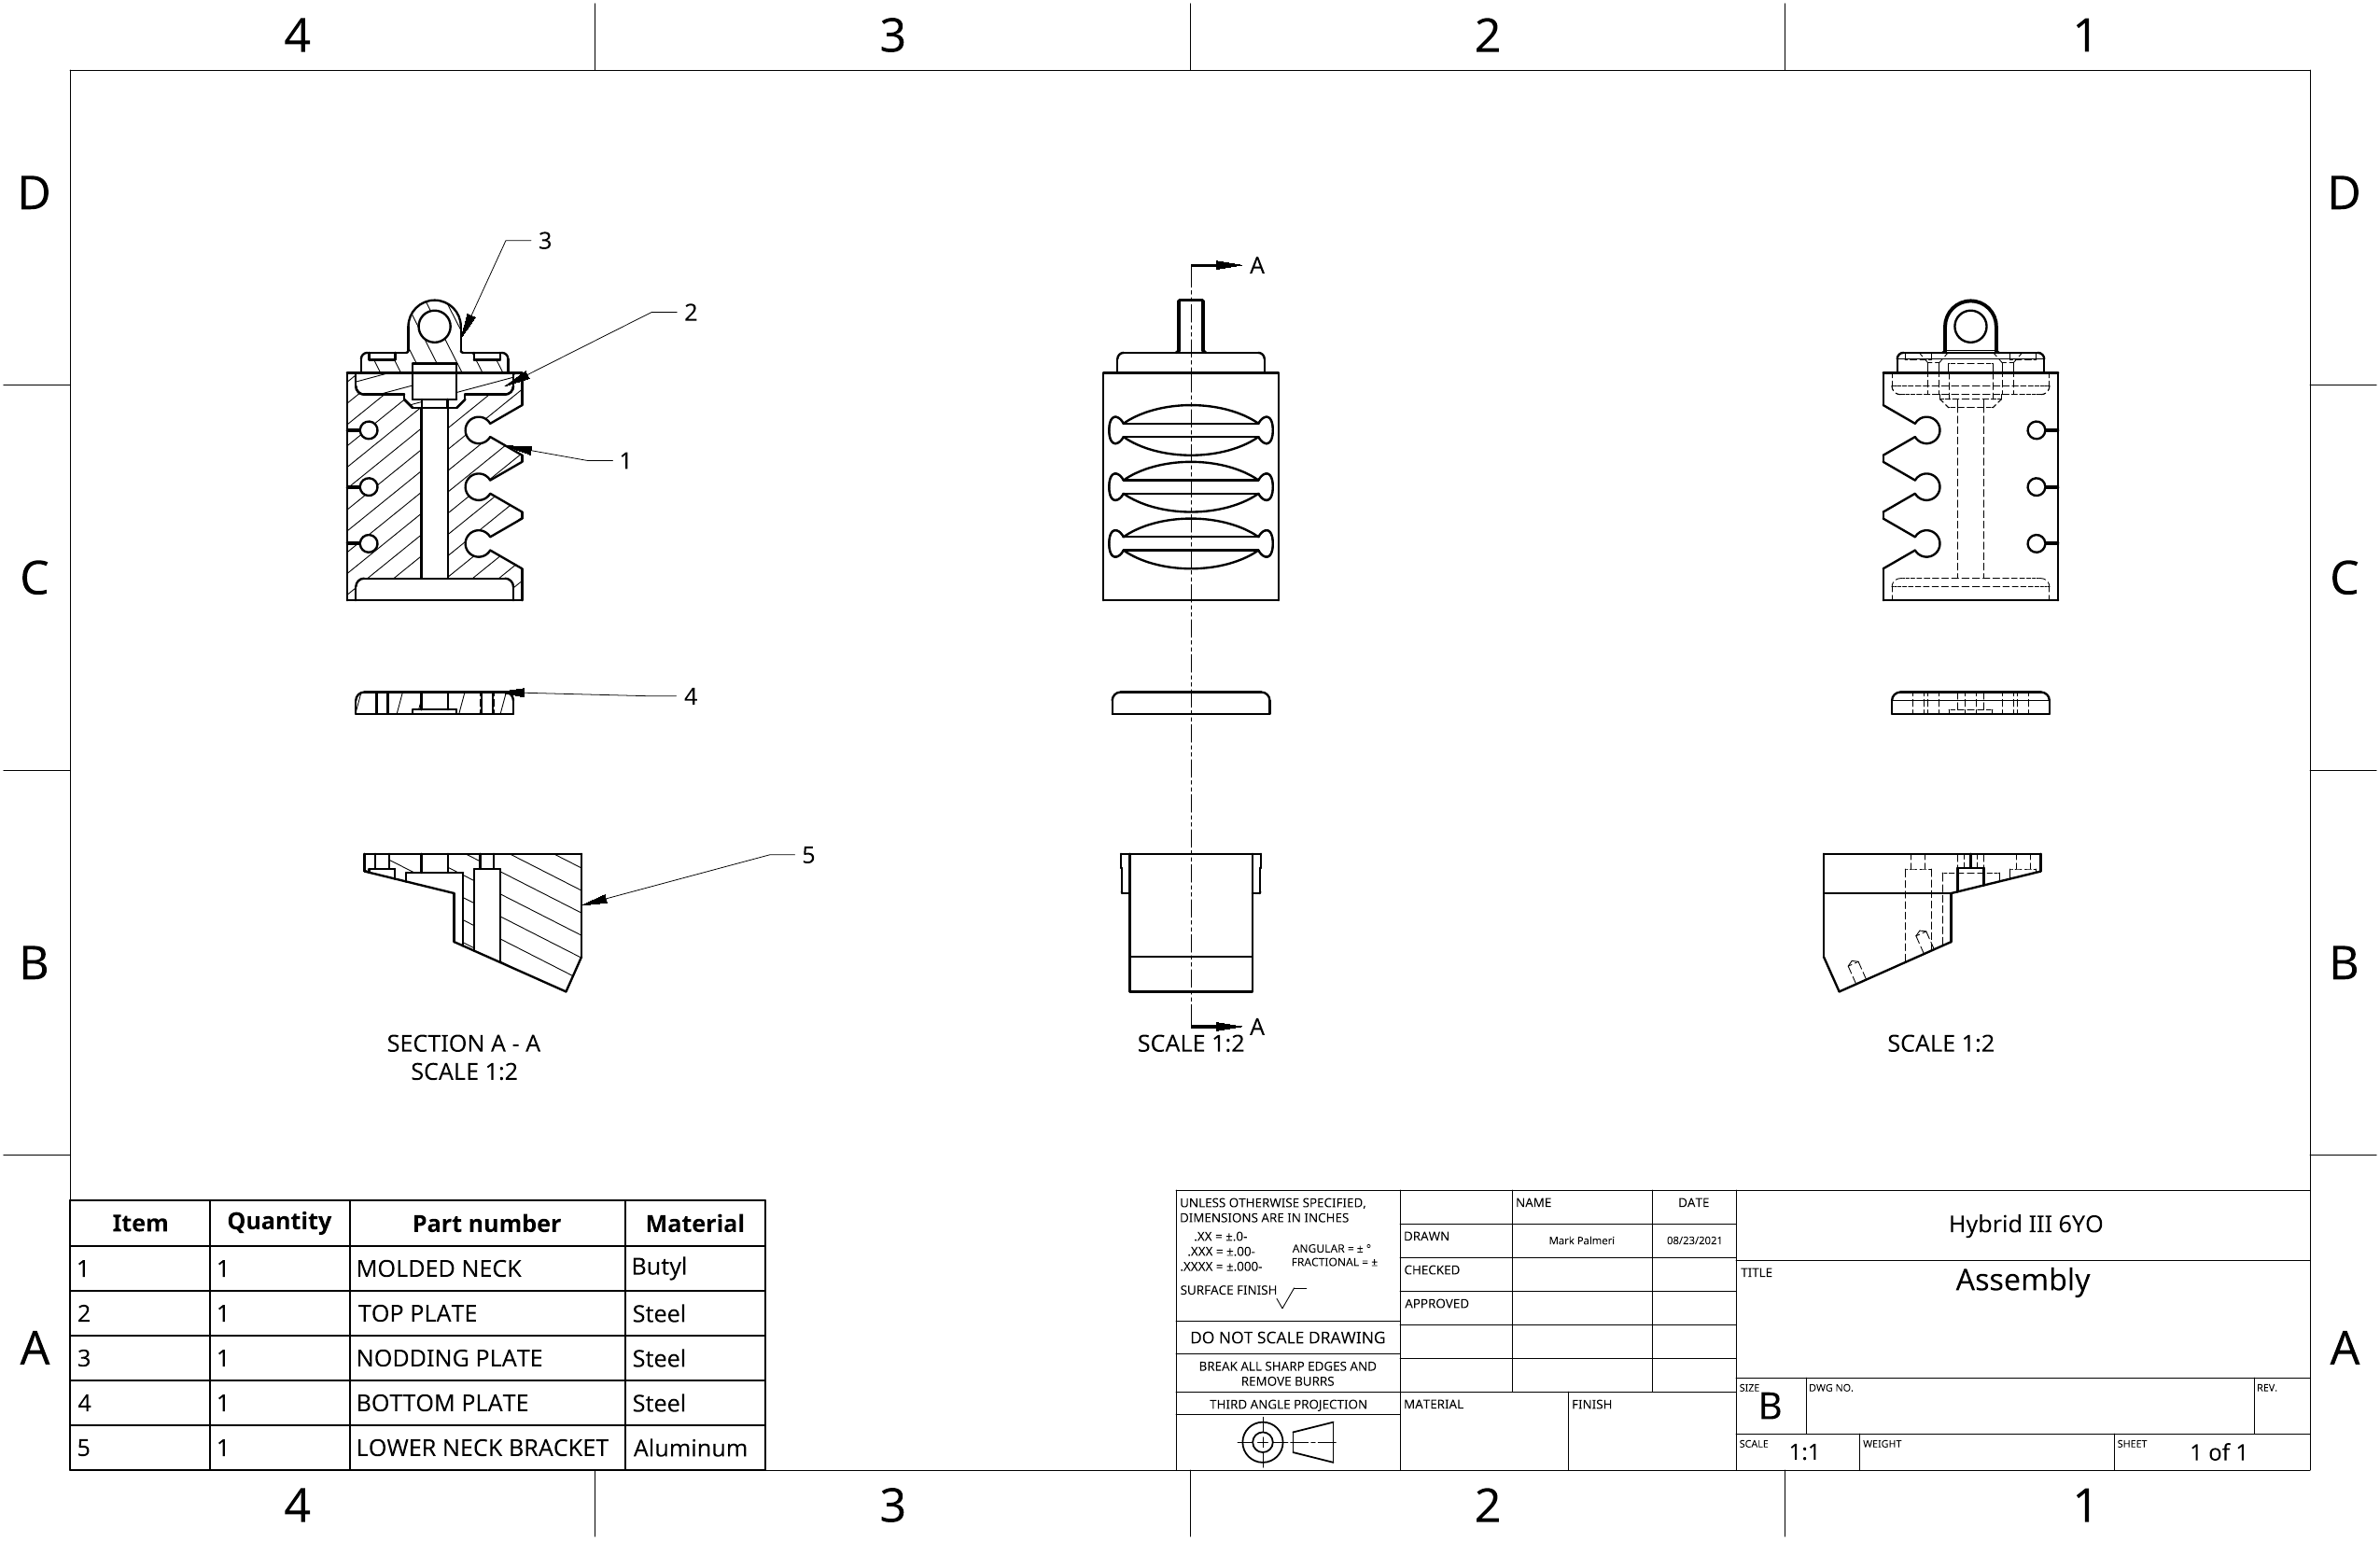
\includegraphics[angle=90,origin=c,width=0.85\textwidth]{AssemblyDrawing.png}}



\end{document}
